\documentclass[border=3pt,tikz]{standalone}
\usepackage{amsmath}
\usetikzlibrary{calc}
\usetikzlibrary{arrows.meta} % for arrow size
\begin{document}

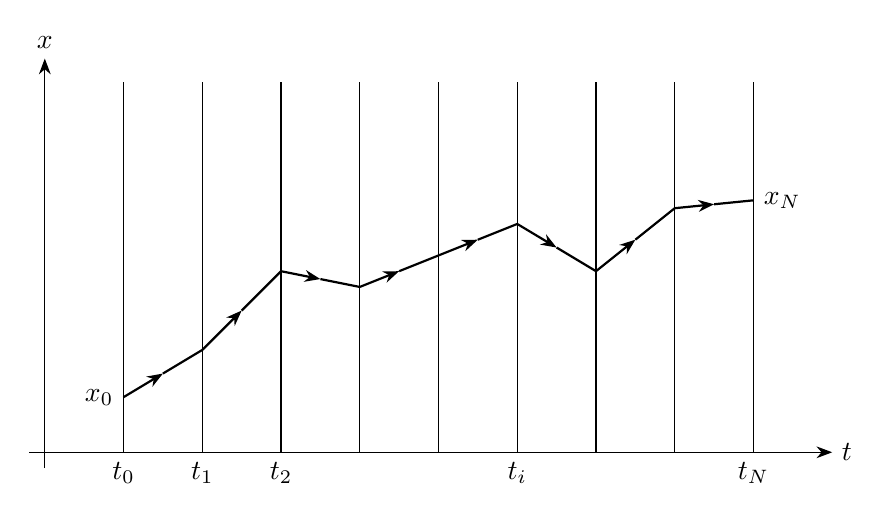
\begin{tikzpicture}[scale=1]
    \usetikzlibrary {arrows.meta}
    \usetikzlibrary {calc}
    
    \draw[, -{Stealth[length=2mm]}] (-0.2, 0) -- (10, 0) node [right] {$t$} ;
    \draw[, -{Stealth[length=2mm]}] (0, -0.2) -- (0, 5) node [above] {$x$};
    
    \foreach \x in {1, 2,..., 9}{
      \draw[] (\x, 4.7) -- (\x, 0);
    }
    
    \node[below] at (1, 0) {$t_0$};
    \node[below] at (2, 0) {$t_1$};
    \node[below] at (3, 0) {$t_2$};
    \node[below] at (6, 0) {$t_i$};
    \node[below] at (9, 0) {$t_N$};
    
    \draw[thick,-{Stealth[length=2mm]}] (1, 0.7) node[left] {$x_0$}-- (1.5, 1.0); \draw[thick] (1.5, 1.0) -- (2, 1.3);
    \draw[thick,-{Stealth[length=2mm]}] (2, 1.3) -- (2.5, 1.8); \draw[thick] (2.5, 1.8) -- (3, 2.3);
    \draw[thick,-{Stealth[length=2mm]}] (3, 2.3) -- (3.5, 2.2); \draw[thick] (3.5, 2.2) -- (4, 2.1);
    \draw[thick,-{Stealth[length=2mm]}] (4, 2.1) -- (4.5, 2.3); \draw[thick] (4.5, 2.3) -- (5, 2.5);
    \draw[thick,-{Stealth[length=2mm]}] (5, 2.5) -- (5.5, 2.7); \draw[thick] (5.5, 2.7) -- (6, 2.9);
    \draw[thick,-{Stealth[length=2mm]}] (6, 2.9) -- (6.5, 2.6); \draw[thick] (6.5, 2.6) -- (7, 2.3);
    \draw[thick,-{Stealth[length=2mm]}] (7, 2.3) -- (7.5, 2.7); \draw[thick] (7.5, 2.7) -- (8, 3.1);
    \draw[thick,-{Stealth[length=2mm]}] (8, 3.1) -- (8.5, 3.15); \draw[thick] (8.5, 3.15) -- (9, 3.2) node[right] {$x_N$};
    \end{tikzpicture}
    \end{document}